\chapter{Locações e Descrição}

Essas são locações e personagens que podem sempre ser encontrados nelas.

\section{Praça Central e a Venda da D. Lurdinha}

A praça central de Barra das Garças é um dos pontos mais movimentados e pitorescos da cidade, cercada por árvores frondosas e canteiros floridos. 

\subsection{A venda de D. Lurdinha}

No coração da praça, encontra-se a famosa venda da D. Lurdinha, uma simpática senhora que vende quitutes regionais e doces caseiros, tornando-se uma referência de acolhimento para moradores e turistas. 
\dperson{D. Lurdinha, proprietária da venda}{
D. Lurdinha é uma personagem singular: em sua infância, afirma ter testemunhado um misterioso objeto cair do céu na floresta próxima, um evento que ela relembra com detalhes vívidos. Ela compartilha essas histórias com quem a visita, afirmando que algo incomum ronda a cidade há décadas. D. Lurdinha é bem-humorada, com um toque de mistério, e sempre parece saber mais do que revela, tornando-se uma importante fonte de informações para os agentes.}{}  


\begin{figure}[hbt]
    \centering
    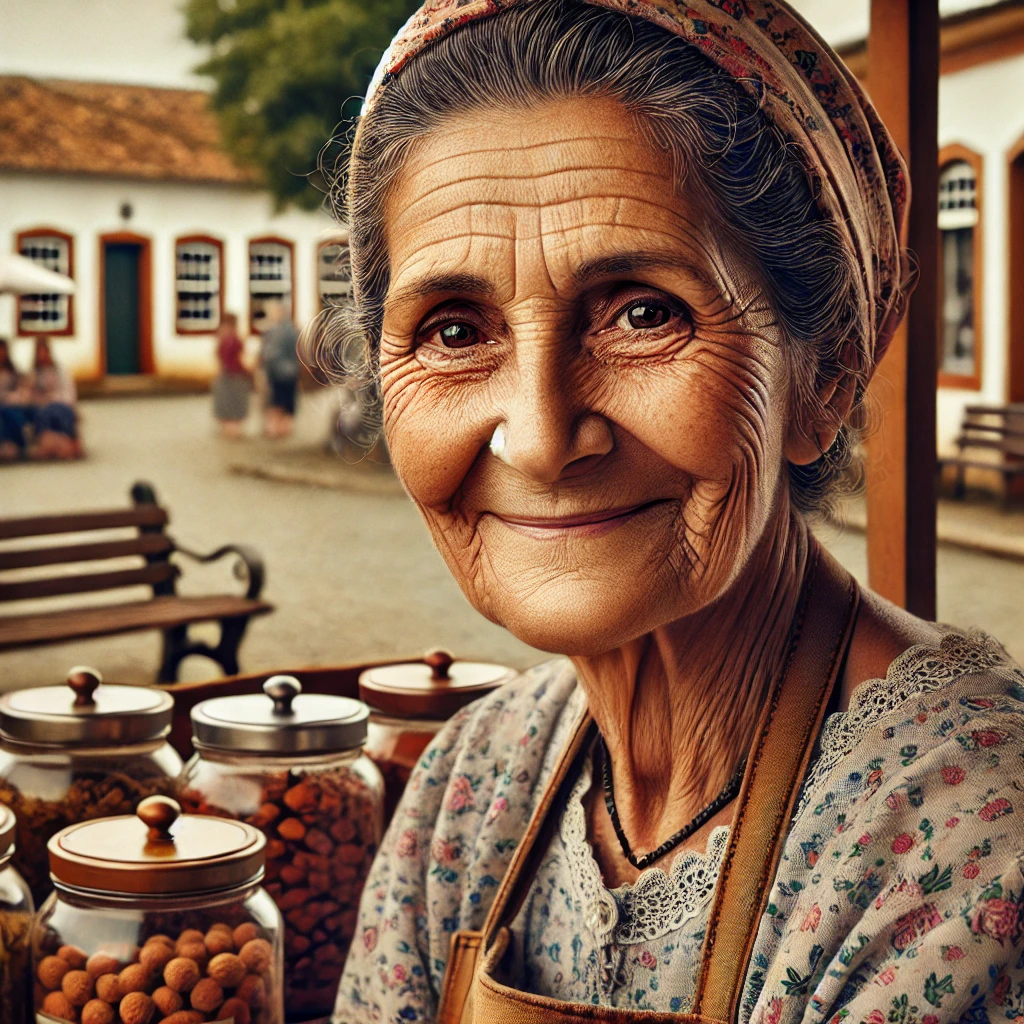
\includegraphics[width=0.5\linewidth]{lurdinha.png}
    \caption{D. Lurdinha}
    \label{figfantasma}
\end{figure}

\subsection{Os jogadores de dominó}


Ao lado da venda, há uma mesa de dominó sempre ocupada por quatro figuras locais, que diariamente jogam e discutem as histórias e mistérios da cidade:

\begin{personagem}[Personagens]
\begin{itemize}
    \item \textbf{Seu Zeca, o Barbeiro}: Um veterano que conhece todos na cidade e costuma afirmar que o cemitério e as cavernas escondem mais do que simples lendas. Ele é observador e já ouviu falar dos intraterrenos.
    \item \textbf{Dona Rosa, a Parteira}: Mulher sábia e respeitada, Dona Rosa acredita no sobrenatural e diz que já viu luzes estranhas na Serra do Roncador. Ela também já fez partos que, segundo ela, foram acompanhados por visões de figuras sombrias.
    \item \textbf{Tonico, o Pescador}: Com sua pele queimada de sol, Tonico diz ter visto OVNIs sobre o rio Araguaia e acredita que são entidades pacíficas. Ele desconfia de Bento e de sua relação com os intraterrenos.
    \item \textbf{Pedro, o Poeta}: Pedro é um boêmio que adora contar histórias poéticas e teorias sobre os portais para outras dimensões. Ele acredita que o ET que caiu está apenas de passagem e tem uma conexão mística com a cidade.
\end{itemize}
\end{personagem}

Cada um deles tem uma personalidade única e suas próprias teorias sobre os eventos misteriosos de Barra das Garças, proporcionando informações e novas perspectivas para os agentes.

\begin{figure}[hbt]
    \centering
    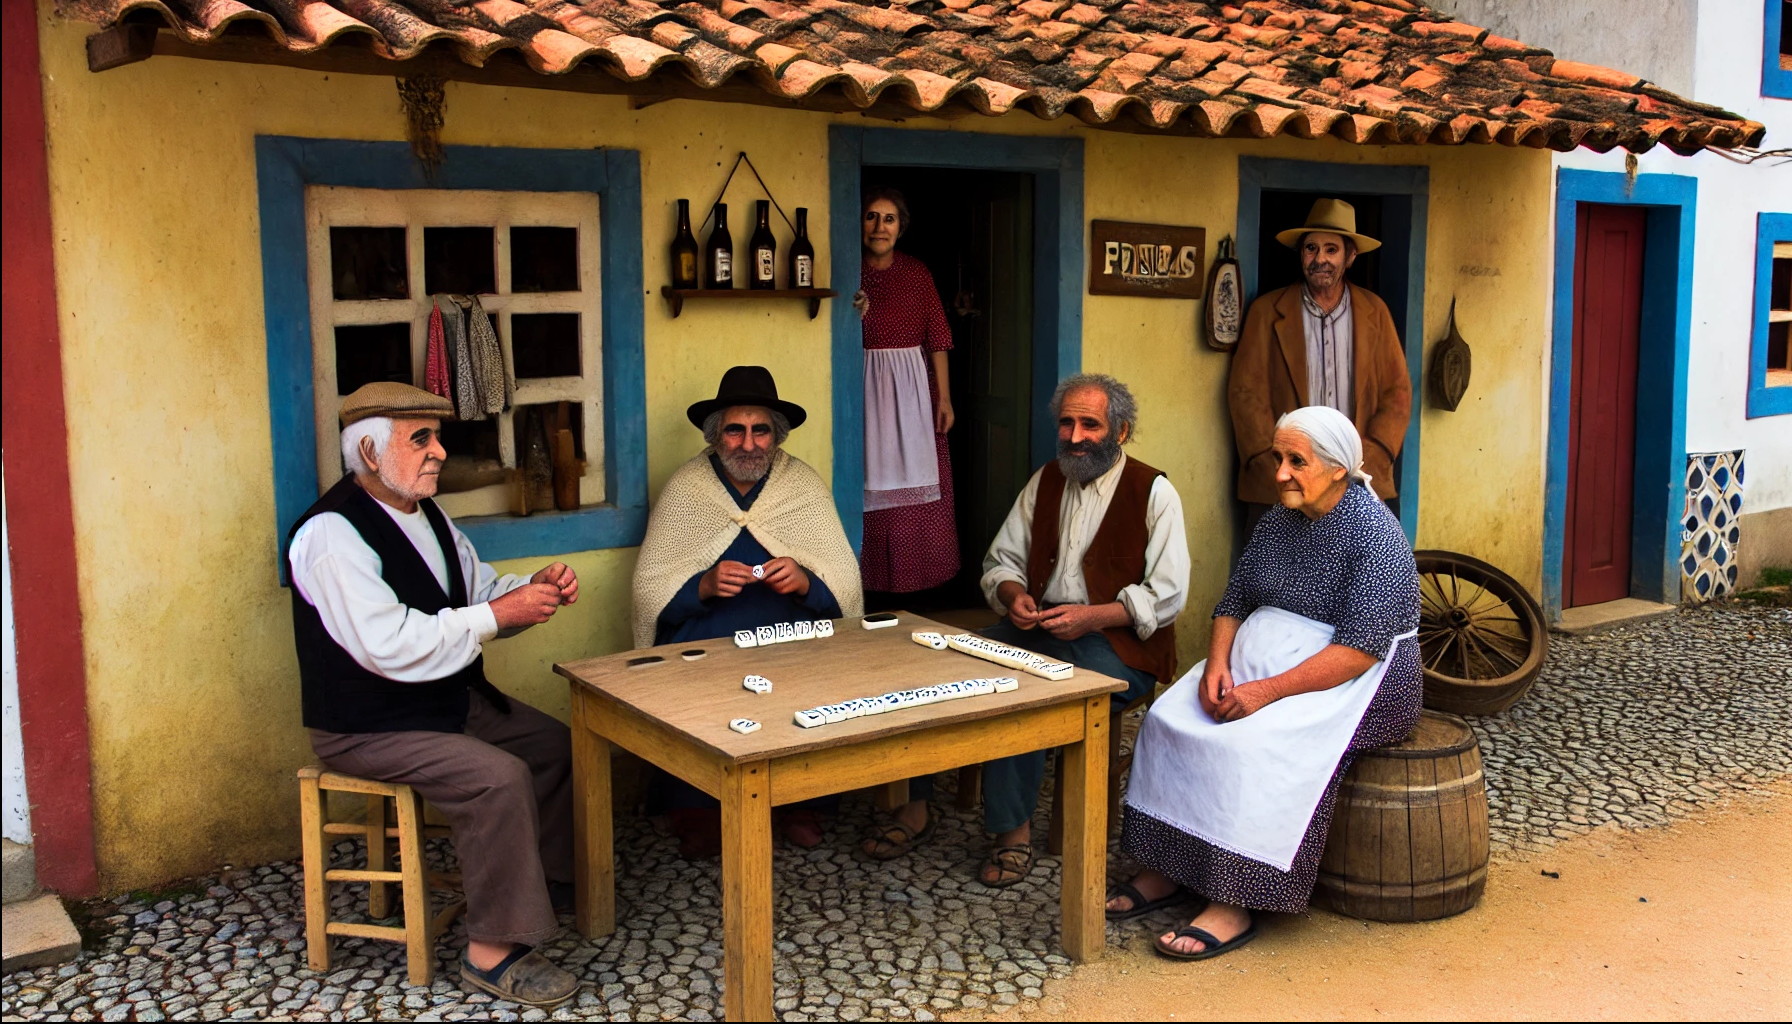
\includegraphics[width=0.5\linewidth]{domino.png}
    \caption{Caption}
    \label{fig:enter-label}
\end{figure}

\section{Interior da Entrada Secreta para o Intraterra}


O acesso ao Intraterra leva a uma caverna com quatro salas, construídas com arquitetura rudimentar. No final do túnel está a \textbf{Sala do Portal}, mas sua porta está trancada por dentro e é impossível entrar. Ela parece ser usada para monitoramento ou controle remoto e possui uma estranha vibração.

\subsection{Salas da Caverna}

\begin{itemize}
    \item \textbf{Sala de Monitoramento}: Contém monitores antigos e uma mesa com anotações em uma linguagem desconhecida. Os intraterrenos usam essa sala para vigiar atividades da superfície. \textbf{Documentos Relacionados}: Notas descrevendo encontros regulares entre humanos da superfície e intraterrenos, incluindo detalhes sobre um grupo liderado por Bento. Essas anotações mencionam o fornecimento de informações sobre atividades na cidade e trocas de recursos em pontos específicos da floresta.
    \item \textbf{Sala de Armas}: Armas primitivas e equipamentos de defesa. Agentes podem reconhecer o estilo similar a relíquias de guerra humanas.
    \item \textbf{Sala de Conferência}: Um espaço para reuniões com uma grande mesa de pedra. Há gravuras nas paredes retratando batalhas antigas com figuras humanoides. \textbf{Documentos Relacionados}: Relatórios sobre estratégias de defesa contra "invasores do céu", que provavelmente referem-se a seres como o ET. O documento também sugere uma aliança de apoio com grupos humanos na superfície.
    \item \textbf{Sala do Portal (trancada)}: Localizada no final do túnel, com portas grossas de pedra que só podem ser abertas por dentro. Os agentes não conseguem entrar, mas devem monitorar a área, pois há sinais de uso recente.
\end{itemize}

\section{Discódromo}

O discódromo sedia uma festa “Mística”, atraindo seguidores de Bento e curiosos sobre o paranormal.

\subsection{Itens e Pistas}

\begin{itemize}
    \item \textbf{Broche de Intraterrenos}: Um pequeno broche em formato de criatura subterrânea, usado pelos aliados de Bento.
    \item \textbf{Convite para Reunião Secreta}: Panfleto sobre uma reunião organizada por Bento e os intraterrenos para discutir a “proteção” da cidade.
\end{itemize}


\begin{personagem}
\subsection{Cláudia, a DJ} Sabe dos encontros de Bento e pode compartilhar informações sobre as atividades do grupo de conspiradores. Ela também ouviu rumores sobre a cidade perdida e diz que alguns dos frequentadores da festa falam sobre ela como um lugar que deve ser evitado a todo custo.
\end{personagem}



\section{Prefeitura}

A prefeitura abriga os registros históricos e é uma importante fonte de dados sobre as atividades incomuns na cidade.

\subsection{Itens e Pistas}

\begin{itemize}
    \item \textbf{Relatos de Avistamentos}: Arquivos sobre luzes e figuras misteriosas vistas na cidade.
    \item \textbf{Mapa Geológico}: Um mapa com informações sobre cavernas e túneis que parecem corresponder aos relatos de eventos recentes.
    \item \textbf{Documentos de Encontro}: Relatórios que descrevem um grupo de residentes da cidade em comunicação com figuras "misteriosas" que se escondem nos túneis subterrâneos. Estes documentos mencionam promessas de proteção em troca de informações e recursos. Há também menção a uma suposta relação entre a cidade perdida e os espíritos obsessores, sugerindo que esses seres possam estar manipulando alguns dos eventos recentes.
\end{itemize}


\begin{personagem}
\subsubsection{Prefeito Antônio de Souza}
\textbf{Nome:} \pindex{Antônio de Souza}
\textbf{Idade:} 58 anos  
\textbf{Descrição:}  
Prefeito Antônio é um homem reservado, que governa a cidade de Barra das Garças com um estilo moderado e diplomático. Ele possui uma postura séria e sempre usa ternos formais, embora mantenha um ar acolhedor para lidar com os cidadãos. O prefeito se preocupa genuinamente com o bem-estar da cidade, mas enfrenta dificuldades para conter os crescentes rumores sobrenaturais. Antônio é casado com a filha do espírito maternal que assombra o cemitério, e o relacionamento com a esposa o torna um homem protetor e discreto, sempre atento ao bem-estar dela.

\textbf{Traços de Personalidade:}
\begin{itemize}
    \item \textbf{Calmo e Diplomático}: Prefere manter a ordem e evita confrontos diretos.
    \item \textbf{Reservado sobre Assuntos Sobrenaturais}: Não gosta de alimentar boatos, mas sente que está perdendo o controle dos rumores.
    \item \textbf{Protetor da Esposa}: Sua esposa tem prioridade em suas decisões, e ele tenta protegê-la de qualquer situação que possa causar-lhe estresse.
\end{itemize}
\end{personagem}


\dperson{Helena de Souza, esposa do prefeito}
{Com 32 anos, Helena é uma mulher linda, amável e bondosa, conhecida por sua gentileza e disposição para ajudar as pessoas da cidade. Ela não sabe que sua mãe faleceu quando ainda era uma criança e que o espírito dela a protege até hoje. Casada com o prefeito, Helena mantém uma presença discreta e evita qualquer atenção pública, preferindo apoiar as causas da cidade por trás das cortinas. Ela tem um forte vínculo com o cemitério, embora não compreenda o porquê.}
{\begin{itemize}
    \item \textbf{Gentil e Caridosa}: É amada na cidade por seu comportamento altruísta.
    \item \textbf{Reservada}: Evita eventos públicos e mantém uma vida privada.
    \item \textbf{Ligação com o Sobrenatural}: Sente-se atraída pelo cemitério e locais místicos, mesmo sem saber o motivo.
\end{itemize}}


\begin{personagem}  

\subsubsection{Subprefeito - Carlos Menezes}

\textbf{Nome:} Carlos Menezes  
\textbf{Idade:} 46 anos  
\textbf{Descrição:}  
Carlos é o subprefeito e uma figura de confiança do prefeito Antônio, conhecido por sua lealdade e eficiência. É um homem prático e pragmático, que cuida dos assuntos administrativos e apoia as iniciativas de desenvolvimento da cidade, especialmente no turismo. Carlos tem uma personalidade resoluta e é cético em relação ao sobrenatural, vendo os boatos como "superstições".

\textbf{Traços de Personalidade:}
\begin{itemize}
    \item \textbf{Eficiência e Pragmatismo}: Resolve os problemas da cidade com rapidez e precisão.
    \item \textbf{Lealdade Inquestionável}: Apoia as decisões do prefeito e faz de tudo para manter a cidade em ordem.
    \item \textbf{Cético ao Sobrenatural}: Considera os boatos sobrenaturais uma bobagem, útil apenas para turismo.
\end{itemize}
\end{personagem}
\begin{personagem}  
 
\subsubsection{Vereador - João "Joca" Alves}

\textbf{Nome:} João Alves, conhecido como "Joca"  
\textbf{Idade:} 42 anos  
\textbf{Descrição:}  
Joca é um vereador simples e próximo do povo, sempre preocupado com as necessidades dos moradores de Barra das Garças. Ele é simpático e amigável, mas extremamente cauteloso com as histórias sobrenaturais que circulam pela cidade. Joca acredita que os boatos causam mais problemas do que benefícios, e tenta moderar as atitudes de Miguel para não alarmar a população.

\textbf{Traços de Personalidade:}
\begin{itemize}
    \item \textbf{Amigável e Popular}: Conhecido por sua proximidade com a comunidade.
    \item \textbf{Prudente e Conservador}: Não gosta de exageros em relação às histórias místicas da cidade.
    \item \textbf{Conflito com Miguel}: Muitas vezes tenta impedir os planos de Miguel para manipular as lendas em benefício próprio.
\end{itemize}
\end{personagem}
\begin{personagem}  
 \subsubsection{Dona Cláudia, a Secretária da Prefeitura}
 
 Conhece bem a história da cidade e suspeita das atividades de Bento. Ela revela que Bento tem buscado mapas das cavernas da região. Dona Cláudia também menciona que muitos registros antigos falam sobre uma cidade perdida e o aeroporto alienígena, frequentemente citados nos documentos mais misteriosos da prefeitura.
\end{personagem}
 
\section{Biblioteca Municipal de Barra do Garças}

\textbf{Descrição:}  
A Biblioteca Municipal de Barra do Garças é uma construção histórica de estilo colonial, situada no coração da cidade, próxima à praça principal. Com paredes de tijolos aparentes e grandes janelas de vidro, o prédio transmite uma atmosfera de mistério e tranquilidade, atraindo tanto moradores quanto visitantes em busca de informações sobre a história e os mitos da região. A biblioteca possui uma coleção variada que abrange desde obras literárias clássicas até documentos sobre o folclore e os eventos sobrenaturais locais.

No interior, a biblioteca é dividida em várias áreas de consulta e pesquisa, com seções dedicadas a literatura geral, periódicos antigos e documentos históricos. A estrutura interna é simples, mas o ambiente é acolhedor e repleto de detalhes místicos, como pequenos quadros com símbolos de proteção e estantes cuidadosamente organizadas. A biblioteca também oferece acesso à internet para consultas digitais, permitindo que os visitantes acessem bancos de dados online e recursos de pesquisa que complementam as investigações locais.

\subsection{Áreas Principais da Biblioteca}

\begin{itemize}
    \item \textbf{Área de Leitura Pública}  
    Um salão amplo e iluminado, com mesas de leitura de madeira dispostas em filas, onde os visitantes podem consultar livros e materiais de estudo. Esta área possui estantes organizadas por categorias que incluem literatura, ciências e mitologia, com uma seção dedicada ao folclore brasileiro e às lendas de Barra do Garças, muito popular entre os visitantes.

    \item \textbf{Arquivo de Documentos Históricos}  
    A seção de documentos históricos está disponível apenas para pesquisadores autorizados e contém registros raros, como mapas detalhados da região, jornais antigos, diários de exploradores e relatos de avistamentos de luzes e criaturas misteriosas. Este arquivo é guardado com segurança, e somente funcionários da biblioteca têm acesso direto às prateleiras, que são fechadas com grades de ferro.

    \item \textbf{Sala de Mapas e Documentação Local}  
    Ao lado do arquivo histórico, esta sala é especializada em mapas e documentos específicos de Barra do Garças e seus arredores. Muitos dos mapas contêm anotações sobre a Serra do Roncador e pontos de interesse onde ocorreram avistamentos misteriosos, e a sala é um ponto valioso para aqueles que investigam atividades sobrenaturais.

    \item \textbf{Seção de Periódicos e Jornais Antigos}  
    Esta seção abriga edições antigas de jornais locais, contendo matérias sobre eventos notórios como o desaparecimento do coronel Percy Fawcett e os primeiros relatos de avistamentos de intraterrenos. Muitos visitantes e pesquisadores buscam essa seção para entender a cronologia dos acontecimentos misteriosos da região.

    \item \textbf{Estação de Acesso à Internet}  
    A biblioteca oferece computadores com acesso à internet para consultas e pesquisas online. Esta área permite que os visitantes acessem bancos de dados, registros públicos, e realizem investigações que vão além dos arquivos físicos. Os computadores são frequentemente utilizados por estudantes e pesquisadores, e alguns visitantes optam por investigar lendas urbanas e teorias conspiratórias por meio de blogs e websites de conteúdo esotérico.
\end{itemize}

\subsection{Personagens da Biblioteca}

\begin{personagem}  
\paragraph{Dona Irene Silva – Bibliotecária Chefe}  
\textbf{Idade:} 62 anos  
\textbf{Descrição:}  
Dona Irene é a responsável pela organização e preservação do acervo da biblioteca. Ela é uma mulher de semblante sereno, sempre disposta a ajudar, mas também reservada sobre as informações que compartilha. Irene conhece profundamente a história de Barra do Garças e as lendas locais, e administra o arquivo histórico com zelo. Embora seja cautelosa, Irene compartilha informações valiosas com aqueles que demonstram interesse genuíno pelos mistérios da cidade.

\textbf{Traços de Personalidade:}
\begin{itemize}
    \item \textbf{Conhecedora das Lendas Locais}: Irene é uma fonte de informações sobre o folclore e os eventos misteriosos da região.
    \item \textbf{Cuidadosa e Atenciosa}: Ela cuida pessoalmente dos arquivos históricos e garante que somente pessoas autorizadas tenham acesso.
    \item \textbf{Reservada e Prudente}: Compartilha informações somente com aqueles que demonstram um interesse genuíno e respeitoso.
\end{itemize}
\end{personagem}
\begin{personagem}  
\paragraph{Gabriel Costa – Jovem Auxiliar}  
\textbf{Idade:} 24 anos  
\textbf{Descrição:}  
Gabriel é o assistente da biblioteca, um estudante de história curioso e apaixonado pelas lendas de Barra do Garças. Ele é responsável por organizar os arquivos e auxiliar os visitantes. Gabriel se interessa pelas teorias sobrenaturais e conspirações locais, e frequentemente direciona os visitantes para seções relevantes. Seu entusiasmo pelo misticismo local torna-o uma ajuda valiosa para quem busca informações sobre o folclore.

\textbf{Traços de Personalidade:}
\begin{itemize}
    \item \textbf{Curioso e Prestativo}: Gabriel adora compartilhar teorias e orientar os visitantes sobre temas misteriosos.
    \item \textbf{Entusiasta de Conspirações}: Ele está sempre atualizado sobre teorias locais e gosta de discutir histórias místicas.
    \item \textbf{Leal a Dona Irene}: Gabriel respeita muito a bibliotecária chefe e ajuda a manter a organização dos arquivos históricos.
\end{itemize}
\end{personagem}

\subsection{Itens e Pistas na Biblioteca}

\begin{itemize}
    \item \textbf{Diário de Joaquim Brandão}: Guardado na seção de documentos históricos, este diário contém informações sobre a investigação de Joaquim antes de seu assassinato, incluindo suas suspeitas sobre Bento Silva.

    \item \textbf{Mapa Anotado da Cidade e da Serra do Roncador}: Na sala de mapas, este documento possui marcações feitas por Joaquim em locais onde Bento realizava encontros suspeitos. As marcações ajudam a traçar os movimentos de Bento e a localizar pontos de interesse para investigação.

    \item \textbf{Arquivo de Periódicos sobre Avistamentos}: Na seção de periódicos e jornais antigos, os personagens podem acessar reportagens e relatos de eventos sobrenaturais que datam de várias décadas, fornecendo uma linha do tempo dos fenômenos misteriosos.

    \item \textbf{Carta Anônima sobre Bento}: Nos documentos antigos, os personagens encontram uma carta endereçada a Joaquim alertando sobre o perigo de investigar Bento, sugerindo que ele poderia estar envolvido com forças "fora deste mundo".
\end{itemize}

\subsection{Interação com a Biblioteca}

A Biblioteca Municipal é um recurso essencial para os personagens que investigam a história e os mistérios de Barra do Garças. Com o auxílio de Dona Irene e Gabriel, os personagens podem descobrir documentos valiosos, acessar a internet para expandir suas investigações, e obter informações que conectam eventos do passado às atividades de Bento Silva e outros envolvidos. O ambiente da biblioteca, repleto de histórias e lendas, incentiva a exploração cuidadosa e oferece várias pistas para desvendar os mistérios da cidade.



\section{Floresta}

Nas margens da cidade e perto do cemitério, há uma área de mata densa onde a nave do ET está escondida. Camuflada com tecnologia avançada, ela emite uma leve vibração detectável apenas com equipamentos especiais.

\subsection{Itens e Pistas}

\begin{itemize}
    \item \textbf{Nave do ET}: Um objeto camuflado, com aparência que se mistura ao ambiente da floresta. A nave só pode ser vista por quem usa equipamento de detecção de radiação ou frequências incomuns.
    \item \textbf{Peça Desgastada}: Uma parte avariada da nave que o ET pede aos agentes para substituir. A peça deve ser recuperada dos intraterrenos.
\end{itemize}


\begin{personagem}  

\begin{itemize}
    \item \textbf{ET}: Explica aos agentes que sua nave sofreu danos e precisa de uma peça específica, que os intraterrenos levaram. Ele pede ajuda para recuperá-la antes que os intraterrenos consigam usá-la contra ele.
\end{itemize}
\end{personagem}

subsection{O Hotel e seus Habitantes}

\subsubsection{Hotel Encanto do Araguaia}

\textbf{Descrição:}  
O Hotel Encanto do Araguaia é o mais antigo da cidade, um casarão colonial reformado que atrai turistas interessados nos mistérios de Barra das Garças. Com uma decoração rústica e tradicional, o hotel preserva um charme antigo, mas também é conhecido por sons misteriosos e fenômenos incomuns que ocorrem à noite. A cozinha do hotel é um ponto de atividades inexplicáveis, e muitos hóspedes já relataram ouvir barulhos estranhos e passos quando tudo deveria estar em silêncio.

\begin{personagem}  
\subsubsection{Dona Celina – Proprietária do Hotel}

\textbf{Nome:} Celina Marques  
\textbf{Idade:} 63 anos  
\textbf{Descrição:}  
Dona Celina é uma senhora elegante e carismática, conhecida por sua hospitalidade e atenção aos detalhes. Ela administra o hotel com dedicação, e embora tenha consciência dos fenômenos que ocorrem à noite, evita discutir o assunto com os hóspedes para não assustá-los. Celina é uma defensora das tradições locais e valoriza a cultura da cidade, mas guarda segredo sobre as atividades estranhas no hotel.

\textbf{Traços de Personalidade:}
\begin{itemize}
    \item \textbf{Hospitaleira e Elegante}: Recebe todos com um sorriso e faz questão de cuidar bem de cada hóspede.
    \item \textbf{Discreta sobre o Sobrenatural}: Prefere não alimentar rumores e ignora os fenômenos quando pode.
    \item \textbf{Ligada à Cultura Local}: Ama a cidade e as tradições locais, contribuindo para preservar a imagem do hotel.
\end{itemize}
\end{personagem}
\begin{personagem}  
\subsubsection{Poltergeist da Cozinha}

\textbf{Descrição:}  
Todas as noites, barulhos inexplicáveis, como talheres se movendo e portas de armários batendo, são ouvidos na cozinha do hotel. Pratos são deixados fora de lugar, e utensílios caem das prateleiras. Os hóspedes curiosos que investigam a cozinha durante a noite frequentemente encontram a cozinha em desordem, mas nunca veem o causador do distúrbio. O poltergeist parece mais brincalhão do que perigoso, mas cria desconforto entre os funcionários e hóspedes.

\textbf{Características do Poltergeist:}
\begin{itemize}
    \item \textbf{Ruídos Altos e Inesperados}: Batidas, passos e barulhos de objetos sendo arrastados.
    \item \textbf{Desordem Visível}: Talheres e pratos mudam de lugar misteriosamente durante a noite.
    \item \textbf{Presença Inquietante}: Provoca sustos, mas não causa danos físicos, preferindo a desordem e o desconforto.
\end{itemize}
\end{personagem}
\begin{personagem}  
\subsubsection{Arrumadeira Tereza}

\textbf{Nome:} Tereza dos Santos  
\textbf{Idade:} 45 anos  
\textbf{Descrição:}  
Tereza é uma mulher de personalidade forte, que cuida do hotel com rigor e eficiência. Ela é uma presença firme, sempre pronta para repreender qualquer um que bagunce os quartos ou corredores. Tereza não se intimida com os boatos de assombração e acredita que o poltergeist é apenas "mais uma coisa" para organizar. Os hóspedes a consideram um pouco rígida
\end{personagem}


\subsection{A Lagoa do Poder}

\textbf{Descrição:}  
A Lagoa do Poder é um local de intensa energia mística, cercado por vegetação densa e distante das trilhas mais frequentadas. A água da lagoa é escura e reflete o céu de forma quase sobrenatural, parecendo mais profunda e misteriosa do que realmente é. Segundo a lenda, a lagoa possui poderes de amplificação espiritual e é usada em rituais por feiticeiros e místicos. Dizem que em noites de lua cheia, a lagoa exibe uma névoa prateada que cobre a água, e quem a toca sente uma onda de energia percorrer o corpo.

\textbf{Características da Lagoa:}  
\begin{itemize}
    \item \textbf{Efeitos Energéticos}: Muitos dizem sentir uma energia poderosa ao redor da lagoa, como se ampliasse percepções e intuições.
    \item \textbf{Lugar de Rituais}: É usada por feiticeiros e bruxas locais para rituais de proteção e conexão com o sobrenatural.
    \item \textbf{Aparições Noturnas}: Estranhas figuras e luzes são vistas em noites de lua cheia, intensificando o mistério da lagoa.
\end{itemize}

\section{Delegacia de Barra do Garças}


A Delegacia de Barra do Garças é um pequeno prédio de tijolos à vista, localizado próximo à praça central da cidade. Com uma fachada discreta, o edifício possui apenas algumas salas para acomodar a equipe policial, um depósito de evidências e uma cela temporária para deter suspeitos. O ambiente é simples e funcional, com móveis desgastados e arquivos antigos empilhados nas prateleiras. A delegacia enfrenta falta de recursos, como muitas outras em pequenas cidades, e conta com uma equipe reduzida. No entanto, o trabalho dos oficiais locais é marcado pela familiaridade com a população e uma abordagem mais pessoal na resolução de casos.

A delegacia está constantemente ocupada com pequenos incidentes locais, como brigas de bar e desentendimentos familiares, mas os rumores sobre atividades sobrenaturais e o aumento de avistamentos de luzes estranhas têm atraído a atenção de algumas figuras inusitadas, levando os policiais a lidarem com novos desafios. Embora alguns policiais sejam céticos quanto às histórias de assombrações e ETs, há uma curiosidade crescente, especialmente entre os mais jovens.

\subsection{Personagens da Delegacia}

\begin{personagem}  
\paragraph{Delegado Pedro Antunes}  
\textbf{Idade:} 48 anos  
\textbf{Descrição:}  
O Delegado Pedro Antunes é o responsável pela delegacia de Barra do Garças. Um homem de presença imponente e experiência na área de segurança, ele mantém uma postura séria e discreta em relação aos rumores sobrenaturais. Pedro é um pragmático, focado em manter a ordem na cidade e evitar alarmismos. Contudo, ele tem um conhecimento detalhado sobre as lendas locais, pois nasceu e cresceu em Barra do Garças, e tem suas próprias teorias sobre os fenômenos, embora prefira não discuti-las abertamente.

\textbf{Traços de Personalidade:}
\begin{itemize}
    \item \textbf{Sério e Discreto}: Prefere lidar com assuntos de maneira formal e raramente se deixa envolver emocionalmente nos casos.
    \item \textbf{Protetor da Comunidade}: Sempre procura resolver conflitos sem atrair atenção negativa para a cidade.
    \item \textbf{Curioso em Relação às Lendas}: Apesar de cético, conhece bem as lendas locais e acompanha os relatos com interesse discreto.
\end{itemize}
\end{personagem}
\begin{personagem}  
\paragraph{Investigador Rafael "Rafa" Martins}  
\textbf{Idade:} 34 anos  
\textbf{Descrição:}  
Rafa é o principal investigador da delegacia e uma das figuras mais populares entre os moradores, graças à sua natureza amigável e ao talento para ouvir e conversar. Ele é um jovem entusiasmado, curioso, e já participou de investigações de casos sobrenaturais por interesse pessoal. Nos últimos meses, Rafa tem mantido um registro informal dos avistamentos de luzes e das histórias sobre o “ET”, e é conhecido por ser o policial que os moradores procuram quando querem discutir temas misteriosos. Ele tem um espírito de aventura e sempre busca entender o que há por trás das lendas.

\textbf{Traços de Personalidade:}
\begin{itemize}
    \item \textbf{Amigável e Acessível}: Rafa é popular na cidade e mantém uma relação próxima com os moradores.
    \item \textbf{Curioso e Investigativo}: Ele se interessa pelos eventos sobrenaturais e frequentemente pesquisa por conta própria.
    \item \textbf{Intuitivo}: É capaz de ler entre as linhas e tem talento para desvendar pistas pouco óbvias.
\end{itemize}
\end{personagem}
\begin{personagem}  
\paragraph{Sargento Luísa Silva}  
\textbf{Idade:} 42 anos  
\textbf{Descrição:}  
Sargento Luísa é uma policial experiente e disciplinada, com uma postura firme e uma personalidade prática. Ela tem pouco interesse pelas histórias sobrenaturais, considerando-as uma distração das questões reais de segurança. Luísa é rigorosa com o cumprimento das regras e é conhecida por seu senso de justiça. Cética em relação aos mistérios de Barra do Garças, vê-se como protetora da comunidade contra o medo e a paranoia, buscando sempre soluções racionais para os casos.

\textbf{Traços de Personalidade:}
\begin{itemize}
    \item \textbf{Rigorosa e Cética}: Luísa não se deixa influenciar por rumores e busca soluções racionais para cada caso.
    \item \textbf{Justa e Leal}: Tem um forte senso de dever e dedica-se a proteger os moradores.
    \item \textbf{Resistente a Pressões Externas}: Não é facilmente influenciada, mantendo uma postura firme.
\end{itemize}
\end{personagem}
\begin{personagem}  
\paragraph{Escrivão Paulo Farias}  
\textbf{Idade:} 50 anos  
\textbf{Descrição:}  
Paulo é o escrivão da delegacia e o responsável por manter todos os registros organizados, o que inclui arquivos de casos e depoimentos. Ele é um homem reservado e organizado, mas possui um lado curioso e está sempre atento às conversas dos colegas sobre os casos sobrenaturais. Paulo possui um vasto conhecimento sobre a história de Barra do Garças e, ao longo dos anos, compilou um acervo pessoal de documentos e reportagens sobre o folclore local, que ele mantém em segredo.

\textbf{Traços de Personalidade:}
\begin{itemize}
    \item \textbf{Organizado e Detalhista}: Responsável por garantir que todos os registros estejam sempre em ordem.
    \item \textbf{Curioso e Reservado}: Tem um acervo pessoal sobre o folclore local, mas compartilha apenas com quem confia.
    \item \textbf{Informante Secreto}: Às vezes revela pistas sobre lendas aos colegas, mas sempre de maneira sutil.
\end{itemize}
\end{personagem}
\begin{personagem}  
\paragraph{Patrulheiro João "Joãozinho" Alves}  
\textbf{Idade:} 27 anos  
\textbf{Descrição:}  
Joãozinho é o patrulheiro mais jovem da delegacia e bastante impressionável. Ele acredita firmemente nos fenômenos sobrenaturais que rondam Barra do Garças e é conhecido por suas histórias exageradas sobre encontros com fantasmas e figuras místicas. Os colegas da delegacia costumam brincar com ele sobre seus medos, mas Joãozinho acredita que a cidade é um ponto de encontro de forças misteriosas. Ele é amigável, prestativo e sempre disposto a compartilhar histórias assustadoras com quem estiver disposto a ouvir.

\textbf{Traços de Personalidade:}
\begin{itemize}
    \item \textbf{Impressionável e Supersticioso}: Acredita em cada história mística que ouve e não esconde isso.
    \item \textbf{Prestativo e Bem-Humorado}: Gosta de ajudar a comunidade e é conhecido por seu bom humor.
    \item \textbf{Narrador Entusiasta}: Sempre tem uma nova história assustadora para contar, encantando moradores e visitantes.
\end{itemize}
\end{personagem}

\subsubsection{Itens e Pistas na Delegacia}

\begin{itemize}
    \item \textbf{Relatórios de Avistamentos}: O Investigador Rafa mantém registros de depoimentos sobre aparições de luzes e figuras misteriosas, muitas vezes compilando as histórias dos moradores em um dossiê informal.
    \item \textbf{Arquivo de Casos Antigos}: O escrivão Paulo tem uma coleção de arquivos antigos que incluem lendas e relatos de atividades incomuns. Em meio aos registros, há menções a uma “cidade perdida” e a figuras misteriosas observadas na Serra do Roncador.
    \item \textbf{Mapa de Avistamentos Recorrentes}: Na sala de investigações, há um mapa com marcas em locais onde avistamentos de luzes foram reportados, muitos dos quais próximos ao cemitério e à Serra Azul.
\end{itemize}

\section{Jornal ``O Araguaia''}

 
``O Araguaia'' é o principal jornal de Barra das Garças, de propriedade do vereador Miguel Rocha. Em circulação há mais de 30 anos, o jornal é conhecido por sua postura conservadora e pelo tom sensacionalista, muitas vezes explorando o folclore e os rumores sobrenaturais da cidade para atrair leitores e fomentar o turismo. Miguel Rocha vê o jornal como uma ferramenta essencial para manipular a opinião pública e promover suas próprias ideias, especialmente o aumento do turismo baseado em lendas locais. 

O jornal possui uma pequena equipe de jornalistas que, embora tenham visões e motivações diferentes, ajudam a construir a narrativa editorial de Miguel, resultando em um periódico com matérias curiosas, mas muitas vezes incompletas ou enviesadas.


\subsection{Vereador - Miguel Rocha}

\textbf{Nome:} Miguel Rocha  
\textbf{Idade:} 53 anos  
\textbf{Descrição:}  
Miguel é um dos vereadores mais influentes de Barra das Garças e tem ideias polêmicas sobre o uso de lendas e boatos para impulsionar o turismo. Ele é o principal criador do plano de "notícias" sobrenaturais e divulga histórias de avistamentos e atividades místicas para atrair visitantes. Miguel é manipulador e astuto, sempre atento aos ganhos financeiros que pode obter com o aumento do turismo.

Como proprietário de ``O Araguaia'', Miguel usa o jornal como uma plataforma para promover seu próprio interesse de manipular o turismo e aumentar seu poder na cidade. Ele é persuasivo e calculista, direcionando a linha editorial do jornal para reforçar as lendas sobrenaturais e as “notícias” misteriosas que alimentam o misticismo da cidade. Miguel é uma figura controversa, e seu jornal frequentemente publica matérias que buscam causar impacto sem uma preocupação real pela veracidade dos fatos.

\textbf{Traços de Personalidade:}
\begin{itemize}
    \item \textbf{Manipulador e Ambicioso}: Constantemente articula planos para lucrar com a cidade.
    \item \textbf{Visionário do Turismo Sobrenatural}: Enxerga as lendas locais como uma oportunidade de atração turística.
    \item \textbf{Persuasivo}: Convence facilmente as pessoas sobre a veracidade dos boatos que espalha.
\end{itemize}


\subsection{Jornalistas de ``O Araguaia''}

\begin{personagem}
    

\paragraph{Jorge, o Jornalista Cansado}  
\textbf{Nome:} \pindex{Jorge Almeida}  
\textbf{Idade:} 52 anos  
\textbf{Descrição:}  
Jorge é um jornalista veterano, cansado e desiludido, que trabalha em ``O Araguaia'' mais por hábito do que por paixão. Ele tem cabelos grisalhos e sempre parece estar com um cigarro apagado nos lábios, além de carregar uma expressão de cansaço. Jorge é preguiçoso e tende a evitar histórias investigativas mais complexas, preferindo escrever sobre assuntos cotidianos e evitar confrontos. Miguel aprecia a falta de ambição de Jorge, pois ele raramente questiona as pautas impostas pelo vereador.

\textbf{Traços de Personalidade:}
\begin{itemize}
    \item \textbf{Desiludido e Preguiçoso}: Evita o trabalho pesado e prefere conteúdos simples.
    \item \textbf{Cínico e Realista}: Jorge não acredita nas histórias sobrenaturais da cidade e as considera apenas uma forma de entretenimento para os leitores.
    \item \textbf{Permanência Conformista}: Trabalha no jornal há anos e é improvável que busque outra ocupação.
\end{itemize}
\end{personagem}
\begin{personagem}
 

\paragraph{Maria Clara, a Jornalista de Esquerda e Blogueira Anônima}  
\textbf{Nome:} Maria Clara Reis  
\textbf{Idade:} 28 anos  
\textbf{Descrição:}  
Maria Clara é uma jovem jornalista idealista e engajada, com uma visão crítica sobre o papel de ``O Araguaia'' em manipular a opinião pública. Ela tem cabelos curtos e óculos redondos, além de um espírito rebelde que a faz entrar em conflito com as pautas de Miguel Rocha. Escreve artigos mais incisivos sobre questões políticas e sociais, mas frequentemente vê suas matérias editadas ou rejeitadas por Miguel. Frustrada, Maria Clara criou um blog anônimo chamado ``Voz do Araguaia'', onde publica as reportagens que não consegue ver no jornal, abordando denúncias e temas progressistas que desagradam ao vereador.

\textbf{Traços de Personalidade:}
\begin{itemize}
    \item \textbf{Idealista e Determinada}: Maria Clara acredita no poder do jornalismo para mudar a realidade da cidade.
    \item \textbf{Crítica e Observadora}: Não se intimida em questionar Miguel e expor as injustiças locais.
    \item \textbf{Ativista Anônima}: O blog ``Voz do Araguaia'' é sua forma de expressar suas visões e expor verdades que o jornal ignora.
\end{itemize}
\end{personagem}



\subsection{Arquivo de ``O Araguaia''}

\textbf{Descrição:}  
O Arquivo de ``O Araguaia'' é um espaço pouco visitado e mal iluminado, localizado nos fundos da sede do jornal. Suas prateleiras abarrotadas de pastas e caixas antigas contêm edições passadas do jornal, recortes de notícias, fotografias, documentos e anotações manuscritas acumuladas ao longo das décadas. O ambiente tem uma atmosfera de decadência, com um cheiro de papel envelhecido e poeira suspensa no ar, criando um cenário nostálgico e sombrio. Embora negligenciado pela equipe do jornal, o arquivo é uma fonte inestimável de informações sobre o passado de Barra das Garças, incluindo histórias esquecidas, investigações abandonadas e rumores sobrenaturais documentados.

O arquivo é mantido em relativo segredo por Miguel Rocha, que prefere que certos documentos permaneçam fora do alcance público. No entanto, sua organização precária e falta de segurança tornam o local acessível para aqueles que ousam explorar em busca de informações ocultas.

\subsubsection{Itens e Documentos no Arquivo}

\begin{itemize}
    \item \textbf{Pastas de Edições Antigas}: Coleções de edições anteriores do jornal, muitas delas repletas de histórias sobrenaturais e lendas locais que, ao longo do tempo, foram usadas para aumentar o fascínio místico de Barra das Garças. Algumas dessas edições contêm anotações à mão de Jorge e Maria Clara, com observações sobre a veracidade das histórias e suas fontes.
    
    \item \textbf{Recortes sobre Fenômenos Sobrenaturais}: Uma coleção de recortes sobre avistamentos de OVNIs, desaparecimentos inexplicáveis e avistamentos de seres místicos, compilados especialmente por Miguel Rocha para alimentar os boatos locais. Há também notas a lápis com comentários questionando a veracidade dos eventos, indicando que nem todos os jornalistas estavam convencidos da autenticidade desses relatos.
    
    \item \textbf{Dossiê ``Expedição Fawcett''}: Uma pasta de documentos sobre o desaparecimento do coronel Percy Fawcett na Serra do Roncador, incluindo recortes de notícias da época e transcrições de entrevistas com moradores antigos. Esse dossiê é uma das relíquias mais antigas do arquivo e é guardado com particular zelo por Miguel Rocha, que vê na história de Fawcett um grande atrativo para o turismo sobrenatural da cidade.
    
    \item \textbf{Fotografias e Negativos Antigos}: Diversas fotografias em preto e branco documentam a evolução da cidade e capturam eventos peculiares que ocorreram ao longo dos anos. Algumas imagens mostram luzes estranhas nos céus e figuras indistintas na floresta ao redor da cidade. Estes negativos são considerados particularmente interessantes por Maria Clara, que acredita que algumas das fotografias nunca foram publicadas por medo de repercussões.
    
    \item \textbf{Documentos de Investigação Inacabada}: Anotações, relatórios e esboços de artigos sobre investigações abandonadas ou censuradas. Jorge, em seus primeiros anos no jornal, tentou desvendar alguns desses mistérios, mas abandonou as investigações após enfrentar pressão de Miguel e desinteresse do público. Esses documentos são úteis para quem busca informações menos filtradas sobre os segredos da cidade.
    
    \item \textbf{Cartas e Denúncias Anônimas}: Um conjunto de cartas enviadas por moradores relatando eventos sobrenaturais, avistamentos de intraterrenos e outros fenômenos misteriosos. Algumas dessas cartas foram publicadas no jornal, enquanto outras foram ignoradas, arquivadas e esquecidas. Muitas delas incluem mapas rudimentares e descrições detalhadas de locais supostamente assombrados ou de interesse místico.
\end{itemize}

\subsubsection{Possíveis Pistas no Arquivo}

\begin{itemize}
    \item \textbf{Mapa Incompleto do Intraterra}: Um esboço antigo que sugere a existência de túneis subterrâneos conectando diversos pontos da cidade. O mapa é rasgado e faltam partes importantes, mas ele indica entradas que podem ser investigadas.
    
    \item \textbf{Carta sobre um Acidente Escondido}: Uma carta de um antigo funcionário público relatando um acidente estranho na serra, envolvendo luzes misteriosas e uma tentativa de encobrir o caso. A carta nunca foi publicada, mas contém informações sobre um local onde restos de tecnologia alienígena poderiam ser encontrados.
    
    \item \textbf{Edição Perdida de ``O Araguaia''}: Uma edição censurada do jornal que menciona uma “conexão perigosa” entre figuras políticas locais e o fenômeno dos intraterrenos. Apenas uma cópia foi preservada e está marcada como “Não publicar” por Miguel Rocha.
\end{itemize}

\section{Bares e Restaurantes}

A cidade de Barra das Garças possui váriosde bares e restaurantes  onde os personagens podem encontrar informações sobre os fenômenos e os personagens enigmáticos da região. Abaixo estão descritos dois bares, dois restaurantes.

\subsection{Bar 'O Tira-Gosto'}

Ponto de encontro local onde os habitantes discutem lendas da cidade. Frequentado por pessoas de todas as idades, o bar é ideal para os agentes ouvirem histórias e coletarem informações. Muitas histórias discutidas no bar mencionam a cidade perdida e um aeroporto secreto para alienígenas que teria sido construído na região, supostamente para facilitar o contato com seres de outros planetas.

\subsubsection{Itens e Pistas}

\begin{itemize}
    \item \textbf{Mapa dos Túneis Subterrâneos}: Um antigo mapa pendurado na parede, revelando a rede de túneis que se conectam ao cemitério.
    \item \textbf{Cartaz da Festa no Discódromo}: Anunciando uma festa temática sobrenatural no discódromo que pode atrair figuras suspeitas.
\end{itemize}

\subsection{Bar ``Lua Cheia''}
\textbf{Descrição:}  
Localizado próximo ao cemitério, o Bar Lua Cheia é um ponto popular entre moradores e curiosos em busca de histórias sobrenaturais. Decorado com temas místicos e esotéricos, o bar é iluminado por luzes baixas e tem paredes repletas de fotos antigas da cidade e de figuras misteriosas, como Percy Fawcett e outras lendas locais. Aqui, os frequentadores discutem abertamente as lendas e os mistérios, e é um ótimo lugar para reunir informações.

\dperson{Sérgio Costa, proprietário}{Um homem na casa dos 50 anos, Sérgio é um entusiasta das histórias de terror e misticismo de Barra das Garças. Ele incentiva os boatos e adora instigar seus clientes com novas teorias, mas mantém um tom cético e trata tudo como entretenimento.
}{}


\dperson{Carla Santos, atendente}{
Carla é jovem e curiosa, sempre ouvindo as histórias dos clientes. Ela é bem informada e adora discutir teorias sobrenaturais, além de contar aos visitantes sobre as aparições e os espíritos que alguns clientes dizem ver ao saírem do bar tarde da noite.
}
{}

\subsection{Bar ``Cachoeira do Roncador''}
\textbf{Descrição:}  
Este bar é localizado próximo à base da Serra do Roncador e é frequentado por moradores e aventureiros que exploram as trilhas e mistérios da serra. Com uma decoração rústica e temática natural, o bar tem mesas de madeira talhadas e oferece uma vista para a floresta, dando ao ambiente um tom calmo e misterioso. Os rumores sobre o discoporto e os intraterrenos são temas comuns entre os clientes.



\dperson{João Carreiro, proprietário}{
Um ex-montanhista e conhecedor das trilhas locais, João está sempre disposto a compartilhar histórias sobre os portais e avistamentos que ocorrem na serra. Ele afirma ter visto luzes estranhas e seres não identificados nas cavernas, mas evita detalhes por medo.
}{}


\dperson{Leandro Maia, atendente}{Leandro é um jovem animado e fã de teorias de conspiração. Ele adora conversar sobre o discoporto e os supostos portais para outras dimensões, alimentando o mistério e incentivando os turistas a explorar a serra.
}{}




\subsection{Restaurante ``Sabor da Terra''}
\textbf{Descrição:}  
Um restaurante familiar e acolhedor, decorado com elementos da cultura local e culinária típica de Mato Grosso. O Sabor da Terra é famoso pela comida regional e é frequentado tanto por moradores quanto por turistas que procuram uma refeição reconfortante. Os boatos sobre o misticismo da região são frequentemente abordados de forma casual durante as refeições.

\dperson{Maria das Dores (Dona Dorinha), proprietária}
{Uma mulher de 60 anos, sempre sorridente e receptiva, Dona Dorinha é uma das moradoras mais antigas de Barra das Garças e conhece as lendas como ninguém. Ela é cuidadosa ao falar sobre o sobrenatural, mas sabe contar histórias intrigantes quando percebe que o cliente tem interesse verdadeiro.}
{}

\dperson{Fabiana Ramos, atendente}
{Fabiana é jovem e trabalha no restaurante desde adolescente. Ela é carismática e gosta de conversar com os turistas, compartilhando histórias sobre o Curupira, o Boitatá e a Lagoa do Poder, histórias que ouviu dos clientes mais velhos.}
{}




\subsection{Restaurante ``Temperos do Cerrado''}
\textbf{Descrição:}  
O Temperos do Cerrado é conhecido por pratos sofisticados inspirados na culinária regional, como peixes frescos e ervas locais. A decoração é elegante, com detalhes rústicos que remetem à cultura indígena. É frequentado por autoridades locais e visitantes importantes, tornando-o um lugar de troca de informações e boatos sobre a política local e mistérios recentes.

\dperson{Carlos Braga, proprietário}
{Carlos é um chef renomado e orgulhoso de suas origens locais. Ele adora conversar com os clientes e possui um conhecimento abrangente sobre as lendas de Barra das Garças, mas evita temas sobrenaturais para não assustar os turistas.}{}


\dperson{Eduardo Santana, atendente}{Eduardo é atencioso e discreto, mas também curioso sobre o sobrenatural. Quando tem oportunidade, ele compartilha histórias sobre o prefeito e suas preocupações com os rumores na cidade, além das estranhas atividades nas cavernas.}{}




\section{Centros de Saúde e o Hospital}

A cidade conta com um conjunto de estabelecimentos de saúde que transcendem o atendimento convencional, cada um com seu próprio mistério e peculiaridade. O hospital, as clínicas e até a clínica veterinária são lugares onde o comum e o sobrenatural se cruzam de maneira sutil, e seus personagens muitas vezes se envolvem em mistérios além dos cuidados de saúde.

\subsection{Hospital Santo Arcano}

O \textbf{Hospital Santo Arcano} é o maior da cidade, localizado em um edifício antigo que, dizem, foi originalmente um convento. De arquitetura gótica, com vitrais coloridos e corredores que parecem se estender infinitamente, o hospital carrega uma atmosfera de mistério. Algumas alas são frequentemente evitadas tanto por pacientes quanto por funcionários, devido a ocorrências inexplicáveis, como luzes que piscam, ecos sem origem e aparições que muitos afirmam ter visto. 

\dperson{Lucas Silveira, médico e chefe da equipe de emergência}{O chefe da equipe de emergência, é um homem calmo e dedicado, mas os que o conhecem bem sabem que ele possui habilidades mediúnicas e ocasionalmente recebe “sinais” do que acontecerá antes de determinados pacientes chegarem. Ele considera essas visões uma maldição, mas as usa para preparar a equipe para os casos mais urgentes.}{} 

\dperson{Rosário, enfermeira}{ conhecida como "A Curandeira" pelos pacientes, tem um conhecimento profundo de ervas e técnicas de cura antigas. Dizem que ela é capaz de sentir a aura das pessoas, sabendo quem está realmente em perigo e quem será capaz de se recuperar. Sua presença é calmante, e alguns acreditam que ela possui um amuleto protetor que mantém o mal afastado.}{}

\dperson{Jonas Ferreira, cirurgião}{ Também possui uma curiosa reputação. Frequentemente, ele realiza cirurgias complexas enquanto recita mantras antigos em latim, acreditando que isso protege tanto ele quanto o paciente. Embora muitos não entendam suas práticas, os índices de sucesso em suas cirurgias são notavelmente altos, e ele é respeitado por toda a equipe.
}{}


\subsection{Clínica Holística Lua de Prata}

A \textbf{Clínica Holística Lua de Prata} é um espaço alternativo, especializado em tratamentos naturais e técnicas de cura espiritual. A clínica oferece terapias com cristais, massagens energéticas e alinhamento dos chakras. As paredes da clínica estão repletas de mandalas, e o ambiente é preenchido pelo cheiro de incenso e o som de músicas suaves.



\dperson{Alice Ventura}{Uma jovem naturopata, é a figura central da clínica. Com uma personalidade calma e uma aparência etérea, Alice é conhecida por suas habilidades de leitura de aura e manipulação energética. Ela tem uma conexão especial com as plantas e acredita que todas as doenças podem ser curadas por meio do equilíbrio entre corpo e espírito. Alice possui um diário secreto em que registra observações místicas de cada paciente, que ela acredita ser fundamental para sua prática. Há rumores de que esse diário possui informações que poderiam revelar conexões ocultas entre pessoas da cidade.}{}

\dperson{Mateus Braga, terapeuta}{
Outro personagem curioso da clínica, é  um terapeuta especializado em hipnose regressiva. Mateus é um estudioso da espiritualidade antiga e acredita que muitos problemas atuais dos pacientes têm raízes em vidas passadas. Ele guarda, em uma gaveta trancada, uma coleção de amuletos supostamente recolhidos dessas regressões, dizendo que cada um pertence a uma "vida anterior" de alguém.}{}


\subsection{Clínica Psicológica Mente Sereno}

A \textbf{Clínica Mente Sereno} é uma clínica psicológica mais convencional, mas seu ambiente é acolhedor e tranquilo. A decoração inclui quadros de paisagens e esculturas de animais espirituais, transmitindo paz e introspecção. A equipe é composta por terapeutas que, de alguma forma, possuem envolvimento com o lado espiritual e esotérico da cidade.



\dperson{Helena Cardoso, psicóloga}{É a psicóloga-chefe e é conhecida por usar uma abordagem integrativa que inclui a espiritualidade como parte do processo terapêutico. De origem cigana, Helena incorpora elementos de sua cultura e prática espiritual em suas sessões, realizando leituras de tarot e interpretando sonhos, que ela acredita serem uma forma de comunicação do inconsciente. Ela possui um baralho que, segundo suas crenças, foi passado por gerações e carrega a energia de seus ancestrais.}{}


\dperson{Felipe Costa}{
Entre os terapeutas, destaca-se o jovem psicólogo e médium, que possui uma habilidade rara de captar sentimentos reprimidos e energias densas. Felipe ocasionalmente menciona “presenças” em algumas salas e utiliza cristais em seu escritório para manter o ambiente limpo. Ele é o único da equipe que consegue lidar com casos de traumas místicos, atraindo para a clínica pacientes que relataram experiências paranormais.}{}

\subsection{Clínica Veterinária Animais Sagrados}

A \textbf{Clínica Veterinária Animais Sagrados} é um lugar especial para os pets da cidade. Acredita-se que a clínica também seja um refúgio para animais com habilidades sensoriais incomuns, como cães e gatos que, segundo os donos, são capazes de pressentir energias negativas ou fenômenos sobrenaturais. A clínica está localizada ao lado de um bosque e emana uma sensação de paz e tranquilidade.

\dperson{Sofia Almeida, veterinária}{A veterinária responsável, é uma mulher calma e intuitiva, que desenvolveu uma conexão profunda com os animais. Sofia é conhecida por utilizar cristais e mantras durante os atendimentos e por tratar de casos em que os animais aparentam estar “sobrecarregados” por energias estranhas. Ela é respeitada na cidade por cuidar de animais que sofreram traumas e diz ser capaz de entender o que eles precisam sem que os donos expliquem muito. Dizem que ela possui um “Livro dos Guardiões” onde registra casos extraordinários envolvendo animais e, supostamente, guarda registros de fenômenos raros. 
}{}

\dperson{Maurícia Correias, assistente}
{Outro personagem da clínica é \textbf{Maurício}, o assistente veterinário e herborista. Maurício trabalha com plantas medicinais e prepara remédios naturais para os animais. Ele possui uma coleção de ervas que colhe nos bosques próximos, acreditando que algumas plantas têm poder de cura especial. Recentemente, ele relatou ter visto espíritos animais protegendo a clínica à noite, e Sofia, embora cética, considera que Maurício pode ter uma sensibilidade rara, que atrai esses “guardiões”.}{}


\subsection{Considerações Finais}

Cada um desses estabelecimentos de saúde é, de certa forma, um elo entre o mundo místico e o real, com profissionais cujas habilidades e peculiaridades estão imersas em elementos sobrenaturais. O hospital e as clínicas tornam-se, assim, locais onde o comum e o extraordinário se entrelaçam, e onde curas, mistérios e segredos guardados oferecem novas dimensões ao já enigmático cenário da cidade.


